\part{Le \textit{low-code} à l'épreuve des interventions techniques}
\setcounter{chapter}{0}

\chapter{La correction des erreurs}

Il existe trois catégories de défis présents sur DiScholEd (et sur toutes les applications web): 
\begin{itemize}[label=\textbullet]
\item Comment corriger les erreurs (\textit{bugs}) ?
\item Pouvons-nous ajouter de nouvelles fonctionnalités ?
\item Comment créer un \textit{design} personnalisé afin que notre application soit reconnaissable ?
\end{itemize}

Nous allons répondre à ces questions au travers d'études de cas et déterminer qui est en mesure de les résoudre. Notre objectif est de définir à qui s'adresse TEI Publisher. Pour rappel, il n'y a pas de développeur expérimenté sur le projet, mais normalement, TEI Publisher utilise le \textit{low-code}, ce qui devrait nous permettre de résoudre nos problèmes sans trop de difficultés.

Les erreurs signalées dans cette section sont générées par notre application et notre code, et non par TEI Publisher. Sur des projets avec moins de documents, ce type d'erreurs peut être facilement résolu, mais cela nécessite néanmoins une recherche approfondie. Nous allons expliquer comment TEI Publisher nous aide dans ce processus avec une étude de cas sur un \textit{bug} de l'application: les index.

\section{Le problème d'affichage des index}

C'est un \textit{bug} présent depuis le développement de DiScholEd. Dans notre application, chaque page de lettre doit afficher à droite du fac-similé un index. L'index comprend un bloc avec les entités nommées qui apparaissent dans le texte.
Il existe deux versions du \textit{bug}: l'un où le texte de la lettre s'ajoute à l'index (cf Figure \ref{fig:schémas04}) et l'autre où le texte apparait dans l'index même s'il n'y a pas d'entités nommées dans la lettre (cf Figure \ref{fig:schémas05}).

\begin{figure}[H]
  \centering
  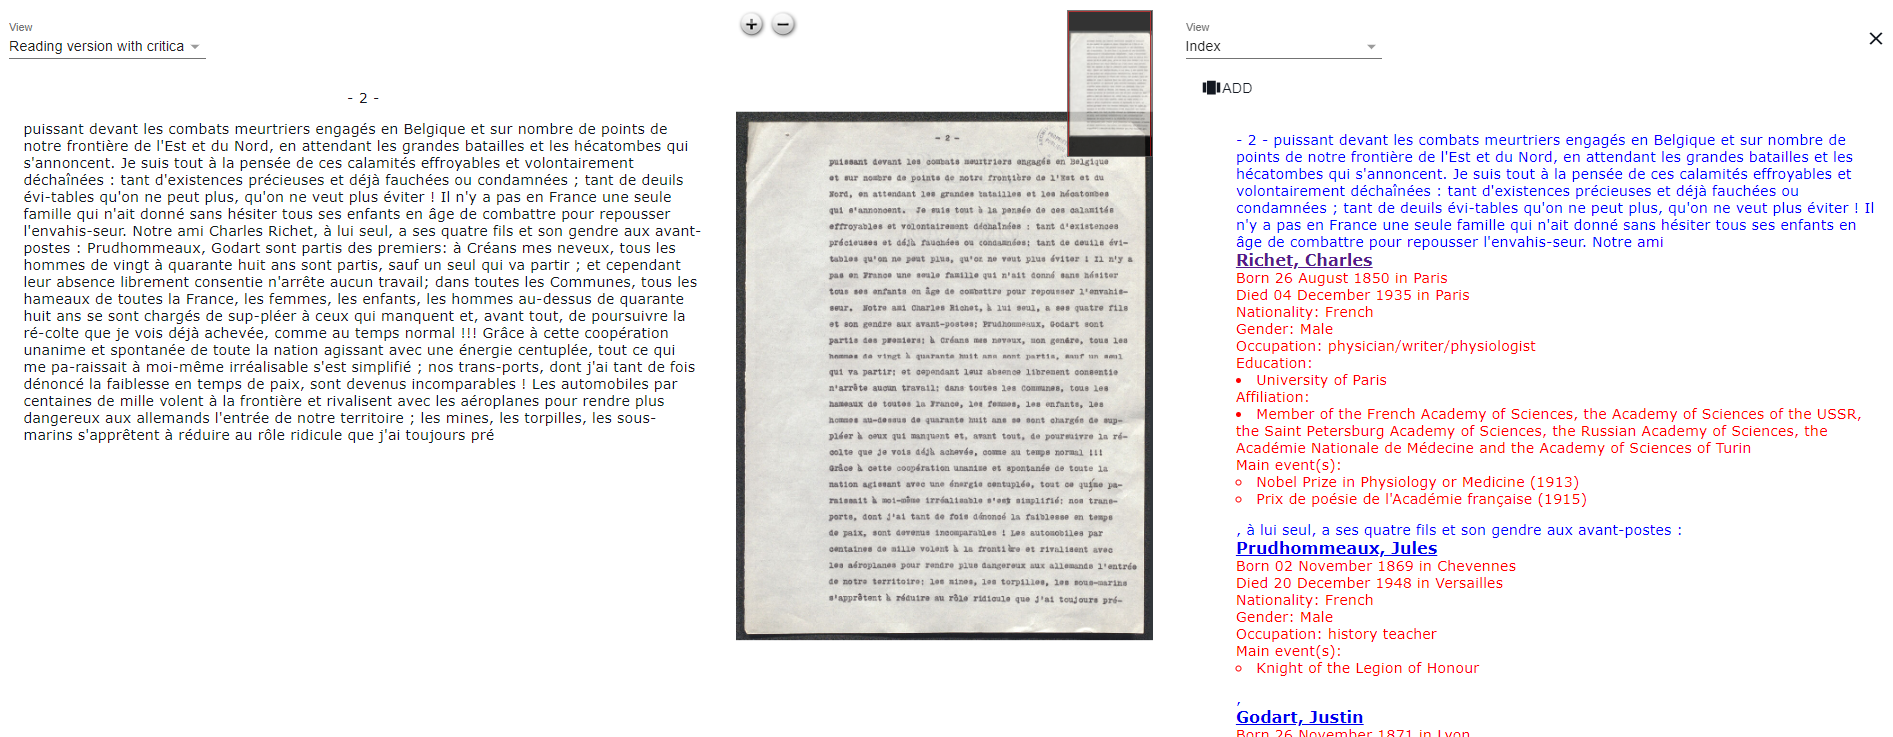
\includegraphics[width=1\linewidth]{schémas/facets text.png}
  \caption{Un exemple d'une lettre, avec le texte inattendu coloré en bleu et les informations d'index correctes colorées en rouge.}
  \label{fig:schémas04}
\end{figure}

\begin{figure}[H]
  \centering
  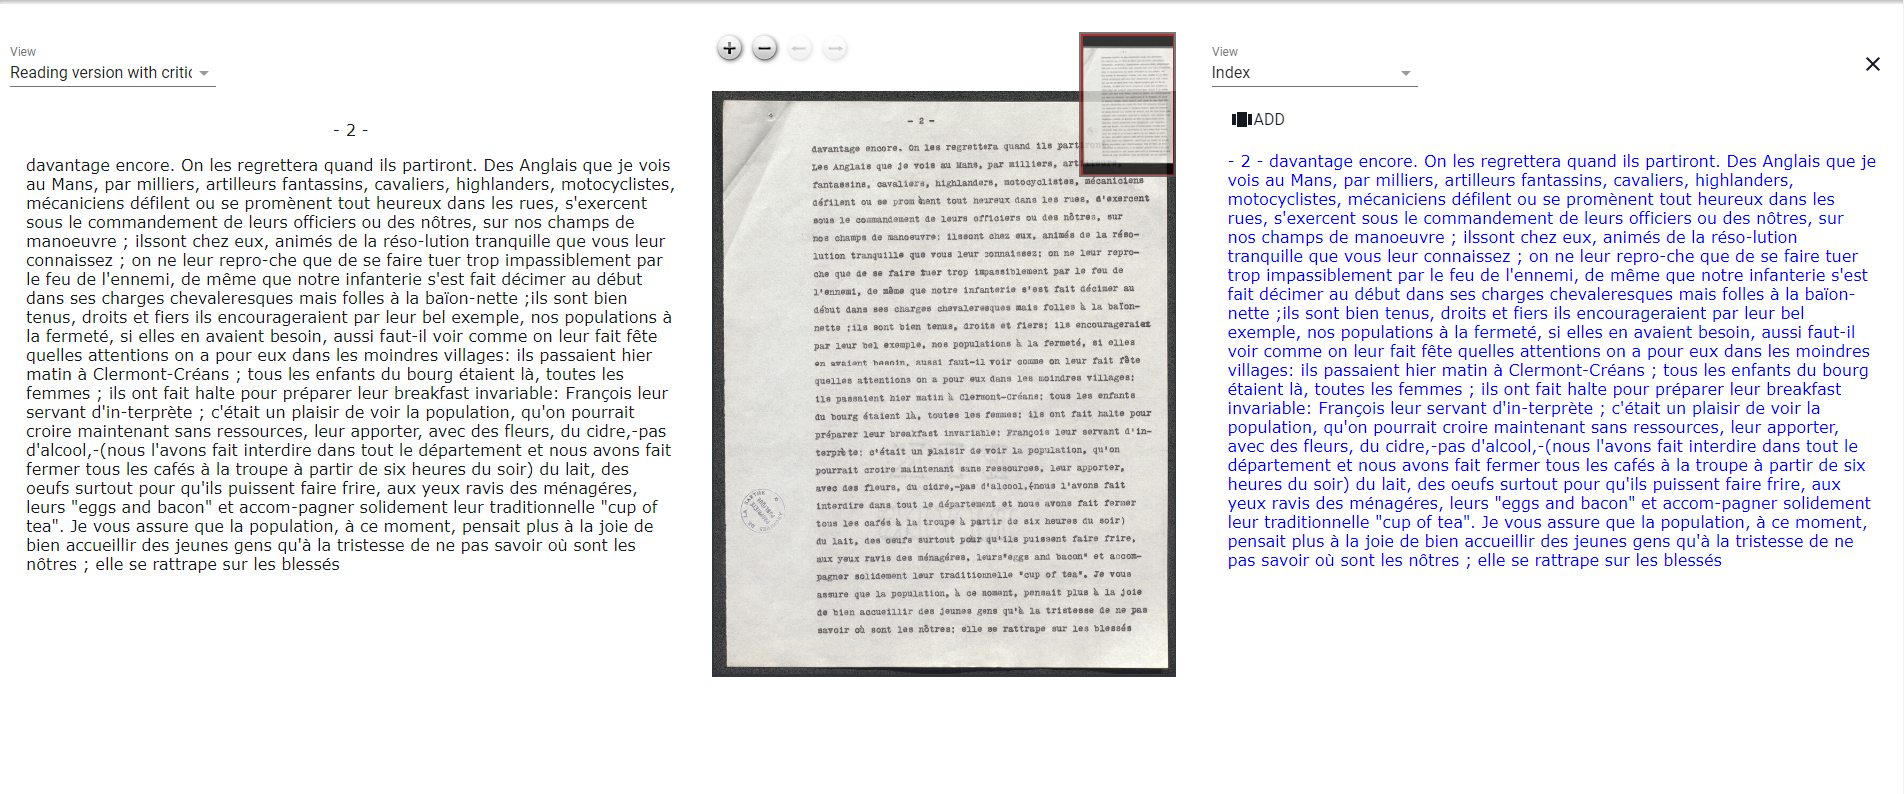
\includegraphics[width=1\linewidth]{schémas/facet_index.png}
  \caption{Un exemple d'une lettre, avec le texte inattendu coloré en bleu alors qu'il n'y a pas d'entités nommées.}
  \label{fig:schémas05}
\end{figure}

Le premier objectif est de comprendre ce qui génère ce problème. Le meilleur moyen est alors de dé-construire l'application et dans notre cas la page web. Il existe deux éléments qui contrôlent l'affichage des index: la page web et l'ODD. La page web appelle le document pour l'insérer dans la page, puis nous appliquons l'ODD au document. Si le problème venait de la page web et de l'HTML alors toutes les pages seraient défectueuses. Dans notre cas c'est donc l'ODD.  

\section{La résolution du problème}

Pour régler ce problème et grâce au \textit{low-code} de TEI Publisher nous pouvons utiliser l'interface graphique pour modifier notre ODD. La règle défectueuse est la balise <p>, qui nécessitait une modification de l'option qui était sur \textit{in-line} et devait être sur \textit{omit}. Cet ajustement a résolu avec succès le premier problème où le texte était dupliqué dans la section de l'index, même s'il n'y avait pas d'entités nommées dans le texte.

Toutefois, bien que le problème précédent ait été résolu, il restait à résoudre la présence du texte et de l'index dans la même section. Un examen plus approfondi a révélé que la balise <p> manquait à certaines pages, car elle faisait partie d'un paragraphe plus large englobant toute la page. Pour résoudre ce problème nous avons décidé d'ajouter des balises <p> d'ouverture et de fermeture accompagnées de commentaires justifiant leur présence. 

La prochaine étape consistait à identifier tous les fichiers où les balises <p> manquaient au sein de leurs sections <pb> (qui définit le début d'une nouvelle page). Dans ce but, un \nameref{script_python_p}(cf. Annexe \ref{script_python_p}) a été créé pour scanner les fichiers, enregistrer leurs noms de fichiers, et noter les balises <pb> correspondantes là où les balises <p> étaient absentes. Un fichier .csv a été généré pour suivre les fichiers problématiques. Ce script a été exécuté avec succès sur les 714 fichiers de l'application, révélant que 108 d'entre eux présentaient le problème identifié, comme nous pouvons le voir dans l’extrait du CSV présent dans la figure \ref{fig:schémas10} :

\begin{figure}[H]
\centering
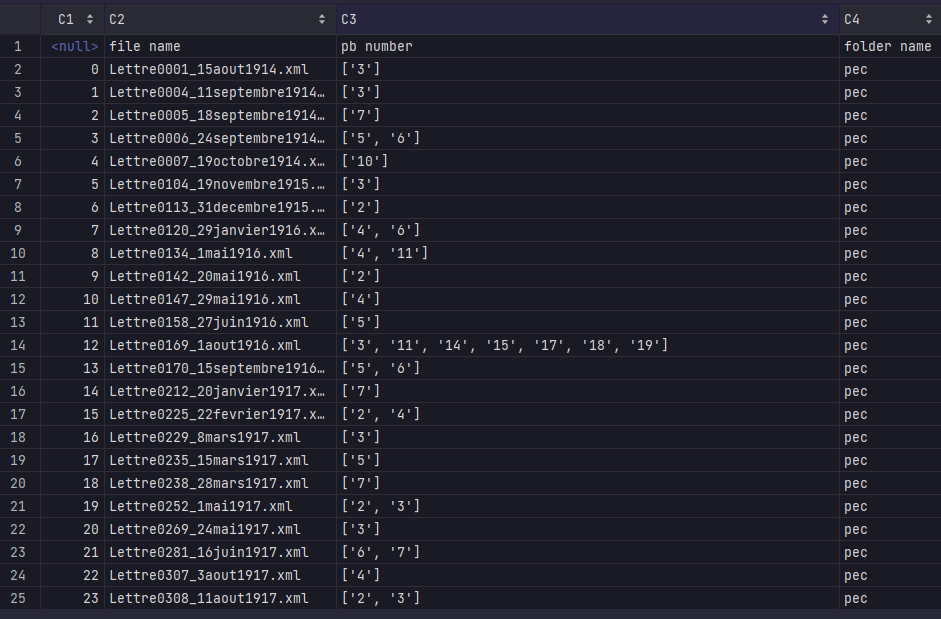
\includegraphics[width=0.75\linewidth]{schémas/script_python.png}
\caption{Le fichier csv qui regroupe tous les documents défectueux par nom de fichier, numéros de pages défectueuses, et nom de dossier.}
\label{fig:schémas10}
\end{figure}

Il a suffi alors pour régler le problème de modifier les fichiers défectueux. Pour ce deuxième cas de figure, TEI Publisher ne nous a pas aidés directement dans la résolution du problème. Nous avons dû trouver la source du problème par nous-mêmes, puis élaborer une solution adaptée à l'ensemble des corpus.

\section{Comment éviter ce bug pour la suite ?}

Le \textit{bug} apparaissait parce que la règle de l'ODD avait besoin d'une balise <p> pour comprendre qu'elle pouvait enlever le texte. Ce n'est pas une erreur qui provient de TEI Publisher, c'est l'un des défis de DiScholEd. En effet, avec autant de corpus, avoir une ODD qui prend en compte tous les cas de figure peut être très compliqué. Il existe deux manières d'éviter ce problèmes : forcer tous les encodages à respecter des règles strictes ou avoir une ODD qui arrive à prendre en considération tous les cas de figure possibles.

Ce \textit{bug} est chose courante dans la programmation et un développeur expérimenté va, avant même d'essayer de coder, réfléchir à tous les cas de figure possibles qui peuvent apparaître et qu'il faut alors prendre en compte. Néanmoins, sur 714 fichiers, c'est très probable d'avoir des oublis de balises. Le problème ne vient pas alors du CMS mais de l'encodage des fichiers. Les éditions numériques de la \textit{Bibliotheca Hertziana} ont par exemple pu éviter ce genre de problème en produisant une démo pour \og{}\textit{study the best way to make the content usable}\fg{}\footcite{epapers4200}.

Les problèmes de correction étaient nombreux, mais pour la plupart faciles à résoudre. Ils témoignent davantage d'une préparation qui n'a pas pris en compte tous les cas possibles d'un CMS défectueux. Pour résoudre ce problème, il n’est pas nécessaire d'avoir un développeur expérimenté, mais simplement la logique de développeur web (quelque chose d'accessible et rapide). 

Le plus souvent, il s'agissait de problèmes liés au HTML, une partie qui, comme l'avait annoncé TEI Publisher, doit être gérée par le développeur de l'application, qui doit avoir des compétences en HTML. La modification de l'ODD est complètement contrôlée par TEI Publisher et nous évite de commettre des erreurs grâce à une interface graphique simple à utiliser. D'ailleurs, des \href{https://www.youtube.com/watch?v=avRO-b2BwUI&ab_channel=wolfgangmm}{tutoriels}\footnote{\textit{TEI Publisher 3.0: Visual ODD Editor}, URL: https://www.youtube.com/watch?v=avRO-b2BwUI (visité le 29/08/2023)}, mis en place par TEI Publisher, sont disponibles pour nous apprendre à bien utiliser l'ODD.\\

Il est impossible pour TEI Publisher de détecter ce type de \textit{bug} ou de fournir des messages d'erreur, car la plupart d'entre eux sont des problèmes graphiques plutôt que des erreurs dans le code. 
Pour palier ces problèmes, TEI Publisher a mis en place une interface graphique, des tutoriels gratuits facilement accessibles, et met à notre disposition des canaux \href{https://app.slack.com/client/T012TH5TPJA/browse-channels/thread/C012YTJP5HB-1654605524.721479}{Slack\footcite{AllChannelsEeditiones}}pour communiquer avec les développeurs. Un autre avantage notable de TEI Publisher réside dans ses <pb-components>, qui nous permettent d'incorporer des éléments essentiels pour une navigation optimale dans notre application.

\chapter{Les nouvelles fonctionnalités de l'application}

\section{Le \textit{bundle} JavaScript}

Lors du développement d'applications web, les développeurs ont souvent recours à différentes bibliothèques, \textit{frameworks} et modules JavaScript pour ajouter des fonctionnalités et de l'interactivité à leurs sites web. Chacun de ces composants est généralement composé de plusieurs fichiers JavaScript. Cependant, le chargement de nombreux fichiers JavaScript séparés peut entraîner une augmentation des demandes réseau et des temps de chargement de page plus lents, ce qui impacte l'expérience globale de l'utilisateur. Pour atténuer ces problèmes, tous les fichiers JavaScript sont compactés dans un \textit{bundle}. TEI Publisher charge son \textit{bundle} depuis internet et donc ne peut pas être modifié, les balises spéciales que nous apporte le \textit{bundle} sont reconnaissables car elles contiennent le préfixe \og{}pb\fg{}, comme <pb-load>, <pb-browse> ou <pb-leaflet-map>.

Lorsque l'on utilise un CMS, l'intérêt est d'avoir accès à des fonctionnalités prêtes à l'emploi dès la création de l'application. C'est un avantage important des CMS restrictifs, l'objectif est d'obliger les utilisateurs à utiliser des éléments qui fonctionnent immédiatement. TEI Publisher, dans son \textit{bundle}, met en place des composants vitaux pour un site web d'éditions numériques, comme le <pb-browse> qui permet de parcourir une collection de documents avec des fonctionnalités de tri et de filtrage.\\

Au travers d'une étude de cas, nous allons expliquer les défis engendrés par la mise en place d'une nouvelle fonctionnalité, en l'occurrence <pb-timeline>, et comment TEI Publisher nous accompagne.

\section{Mise en place d'un composant: <pb-timeline>}

Une balise spéciale <pb-timeline> est utilisée pour afficher une chronologie de tous les fichiers d'une collection. Cette fonctionnalité est une nouveauté de la dernière version de TEI Publisher. Pour implémenter le <pb-timeline> dans la plateforme, une règle d'API personnalisée doit être créée. Pour <pb-timeline> un règle de l'API a été conçue pour renvoyer un objet JSON, où chaque propriété représentait une date ou le marqueur spécial \og{}?\fg{} indiquant des ressources non datées. Chaque entrée contenait une valeur correspondant à un nombre de ressources ou à un objet avec les propriétés \textit{count} et \textit{info} (les balises <a> qui font les liens vers les documents).

Alors que d'autres applications utilisaient une règle XQuery pour générer la chronologie dans un fichier XML, nous avons opté, pour l'utilisation d'un \nameref{script_python_timeline}(cf. Annexe \ref{script_python_timeline}) pour produire un fichier XML contenant les informations nécessaires, comme cela peut s’observer dans le fichier \nameref{xml_file_timeline}(cf. Annexe \ref{xml_file_timeline}). Ce fichier XML est ensuite transformé par l'API au format JSON attendu pour le <pb-timeline>.

Lorsque la page web se charge, l'élément <pb-timeline> appelle l'API et reçoit un fichier JSON, il crée alors un histogramme. Cet histogramme utilise le fichier JSON et, pour chaque année, il reçoit le nombre de documents correspondants. Il peut alors, pour chaque année, créer une barre qui, lorsqu'elle sera survolée avec la souris, pourra afficher les liens vers les documents l'année survolée.

\begin{figure}[H]
\centering
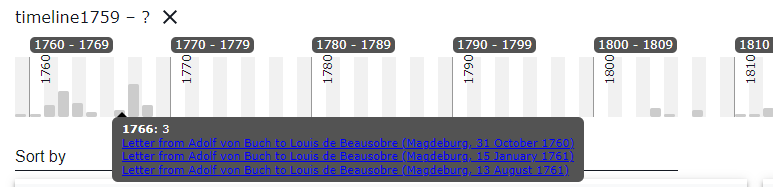
\includegraphics[width=0.75\linewidth]{schémas/timeline.png}
\caption{Un exemple d'un élément <pb-timeline> et de l'année 1766 du corpus \og{}Lettres et textes : Le Berlin intellectuel des années 1800\fg{}}
\label{fig:schémas06}
\end{figure}


\section{L'importance des éléments du CMS}

Pour réussir à utiliser les éléments propres à DiScholEd, il faut se référer à la documentation\footcite{TEIPublisherWebcomponents}. Les éléments de cette documentation sont spécifiques à TEI Publisher, ce qui constitue l'une des raisons qui pourraient nous inciter à opter pour ce CMS. Les éléments de TEI Publisher sont regroupés dans un ensemble appelé \textit{bundle}. Pour les intégrer dans notre application, il est nécessaire de se référer à la documentation, ou bien il est envisageable de télécharger des applications qui l'utilisent afin d'examiner et de comprendre comment ces éléments s'intègrent dans l'application. Par exemple, la timeline est utilisée par l'application : \href{https://www.briefedition.alfred-escher.ch/briefe/}{\textit{Briefe Editions} \footcite{EditionLettresEdition}}. 

La documentation peut être parfois lacunaire et les démos proposées ne sont pas fonctionnelles. C'est pourquoi pouvoir télécharger les applications est très important et permet de mieux comprendre comment l'élément fonctionne dans l'application. La mise en place de la \textit{timeline} demande des compétences élevées en développement et est l'un des éléments les plus compliqués à mettre en place. 

Il est aussi possible de s'affranchir du CMS et de faire comme pour le projet AGODA et \og{}\textit{implement components developed in the framework of TIME-US, and create new ones.}\footcite{puren:hal-03623351}\fg{}

Pour DiScholEd, l'utilisation du script Python pour créer les fichiers XML des timelines était obligatoire. En effet, les différences d'encodage dans les différents corpus nous ont empêché d'utiliser le XQuery officiel de TEI Publisher que \href{https://www.briefedition.alfred-escher.ch/briefe/}{\textit{Briefe Editions} \footcite{EditionLettresEdition}} utilise, par exemple.

La <pb-timeline> est un élément important : qui en plus d'améliorer le \textit{design} du site nous donne un aperçu rapide de la répartition dans le temps des documents. Néanmoins, sa mise en place demande de fortes connaissances en XQuery ou Python et est donc réservée à des développeurs.

Les éléments du \textit{bundle} jouent un rôle central dans la création d'une application de qualité, mais leur manipulation exige une solide expertise en informatique. Parfois, il est nécessaire de démonter d'autres applications pour parvenir à comprendre leur fonctionnement, faute de documentation adéquate. La mise en place de la \textit{timeline} n'est pas nécessaire pour les corpus suivants : le \og{}Journal des guerres napoléoniennes\fg{} et \og{}Ma Guerre 1914-1918\fg{}, qui ne comportent qu'un seul texte. En revanche, les cinq autres corpus contiennent généralement plus d’une centaine chacun, et avoir une répartition temporelle de tous les documents revêt une grande importance.

Certaines fonctionnalités de TEI Publisher sont trop complexes à mettre en œuvre pour les chercheurs. Cependant, ces éléments seraient moins pertinents pour leurs projets, car ils concernent souvent des ensembles de données plus restreints. TEI Publisher, bien qu'il se veuille accessible à tous, notamment aux chercheurs, n'en reste pas moins complexe à utiliser. Il est impossible de mettre en place des fonctionnalités complexes avec le \textit{low-code}, car cela requiert de la programmation en XQuery et une compréhension approfondie du fonctionnement de l'application. Pour les projets avec moins de documents, TEI Publisher permet effectivement de développer rapidement une application bien conçue. L'exemple du projet DiScholEd montre que la prestation d'un développeur ou de l'équipe de TEI Publisher est nécessaire pour développer l'application dans des conditions optimales.\\

Comme nous l'avons mentionné, TEI Publisher se situe quelque part entre la restriction et la liberté. Il convient aux projets qui n'exigent pas de fonctionnalités avancées, mais à mesure que le projet prend de l'ampleur, le besoin d'un véritable développeur devient de plus en plus crucial. Avec l'augmentation de la taille d'un projet, l'importance d'un bon \textit{design} devient cruciale.  

\chapter{L'amélioration de l'expérience utilisateur (UX)}

Les améliorations de l'application consistent en toutes les modifications apportées au \textit{design} de l'application. Par exemple, la mise en place des \textit{splash} est une amélioration de DiScholEd. L'UX (Expérience Utilisateur) d'une application web, lequel est étroitement lié à son \textit{design}, contrôle le ressenti global de l'utilisateur tout au long de son interaction avec l'application. L'UX englobe les défis d'accessibilités, d'esthétiques visuelles et d'ergonomies.

\section{Les fonds d'écran \textit{Splash} ou écrans de chargement}

Pour chaque collection, nous avons mis en place un arrière-plan d'écran de démarrage qui est une image de chargement utilisée comme arrière-plan. Lors du chargement d'une page, un écran de démarrage correspondant est appelé et affiché pendant que la page est en cours de chargement. Au début de mon stage, l'application n'avait pas d'écran de démarrage implémenté (cf Figure \ref{fig:schémas09}). Par conséquent, lors du chargement de la page, plusieurs informations aléatoires, telles que les langues disponibles dans l'application, étaient affichées au lieu d'un écran de démarrage spécifique.Nous avons alors mis à jour toutes les images des collections et des \textit{splash} avec des versions de meilleure qualité, enrichissant ainsi davantage l'expérience utilisateur (cf Figure \ref{fig:schémas07}-\ref{fig:schémas08}).

\newpage

\begin{figure}[H]
\centering
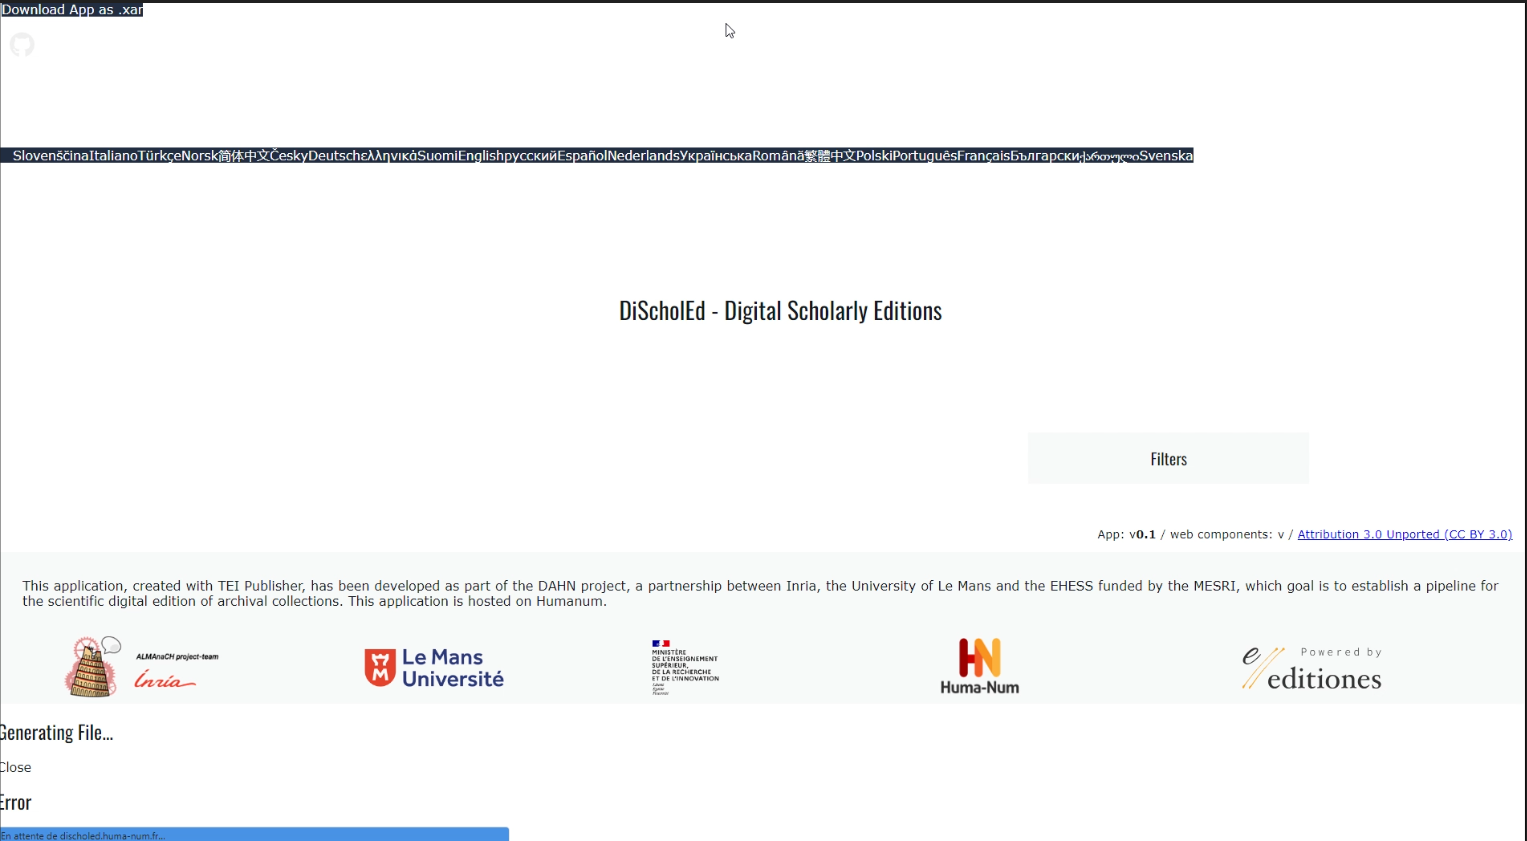
\includegraphics[width=0.75\linewidth]{schémas/old_splash.png}
\caption{Première version du \textit{splash} non fonctionnelle}
\label{fig:schémas09}

\centering

\includegraphics[width=0.75\linewidth]{schémas/new_splash.png}
\caption{Nouveau \textit{splash} de l'application}
\label{fig:schémas07}

\centering
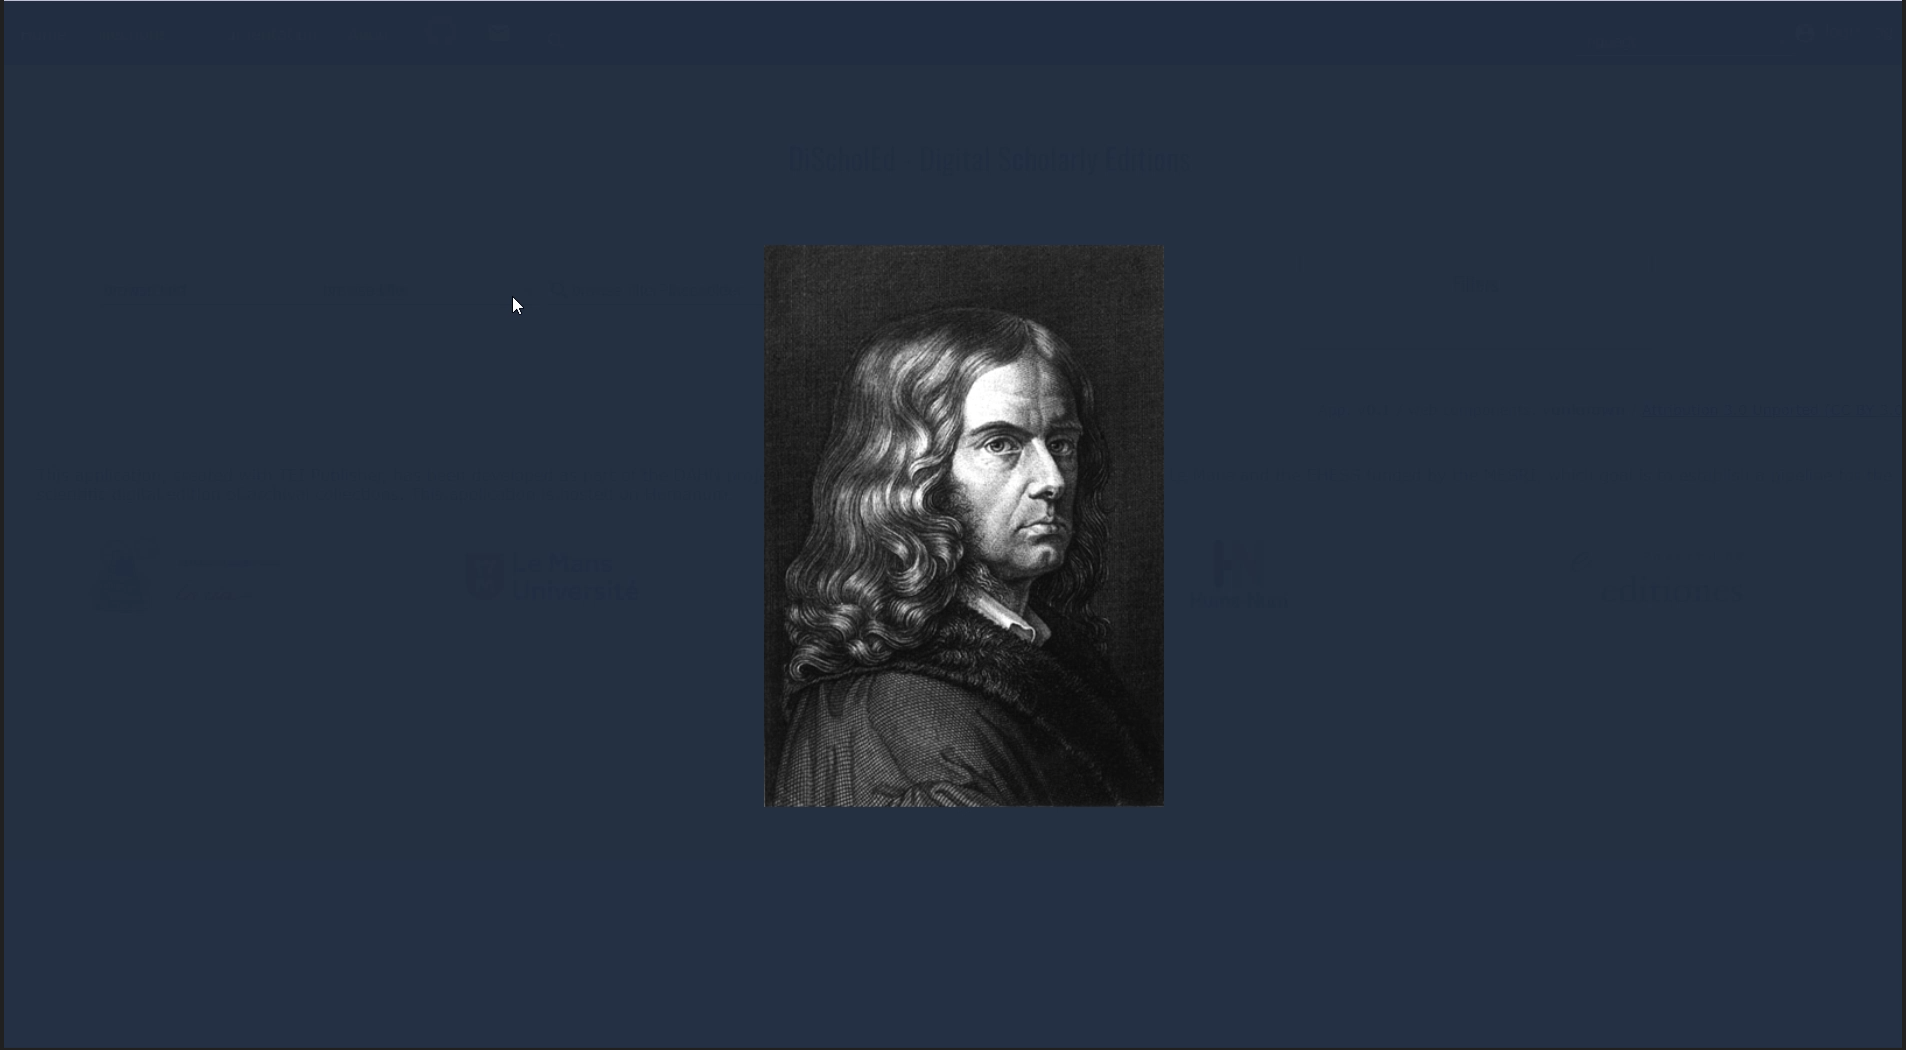
\includegraphics[width=0.75\linewidth]{schémas/new_splash_bi.png}
\caption{Nouveau \textit{splash} d'une collection}
\label{fig:schémas08}
\end{figure}

\section{L'importance du \textit{design} dans une application web}

Il est essentiel d'offrir une expérience utilisateur (UX) à la fois conviviale et mémorable. C'est la première impression que l'application laisse sur les utilisateurs, car elle constitue la façade de notre application et leur première interaction avec elle. Un site web doit être intuitif et facile à utiliser. DiScholEd, en tant que projet axé sur les éditions numériques, cible principalement un public de chercheurs. Une certaine connaissance en HTML est nécessaire pour la construction de notre site, car nous devons mettre en valeur sept corpus différents. Pour ce faire, nous avons mis en place plusieurs améliorations, notamment un carrousel des corpus sur la page d'accueil, une refonte du \textit{design} des pages de corpus et une amélioration de la qualité des images de présentation des corpus (cf Figure \ref{fig:schémas11}-\ref{fig:schémas13}).

\begin{figure}[H]
\centering
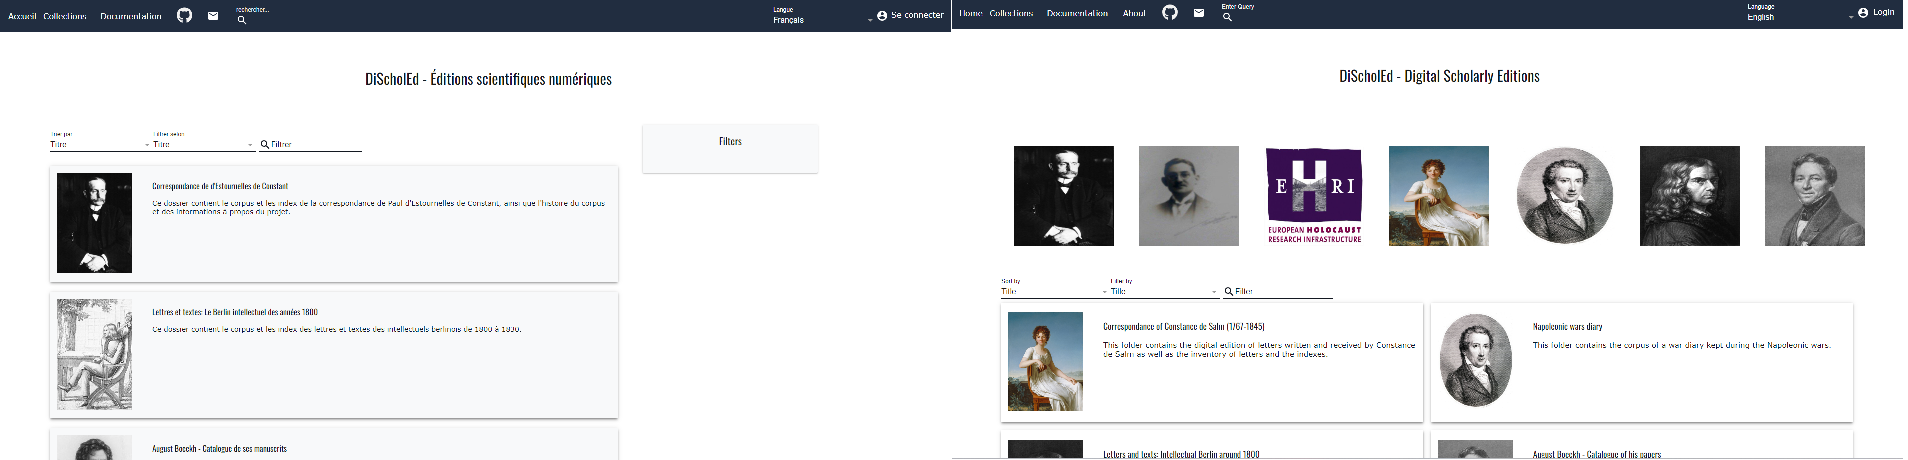
\includegraphics[width=1\linewidth]{schémas/carrousel.png}
\caption{ La page d’accueil sans le carrousel (gauche) puis avec (droite) }
\label{fig:schémas11}
\end{figure}

\begin{figure}[H]
\centering
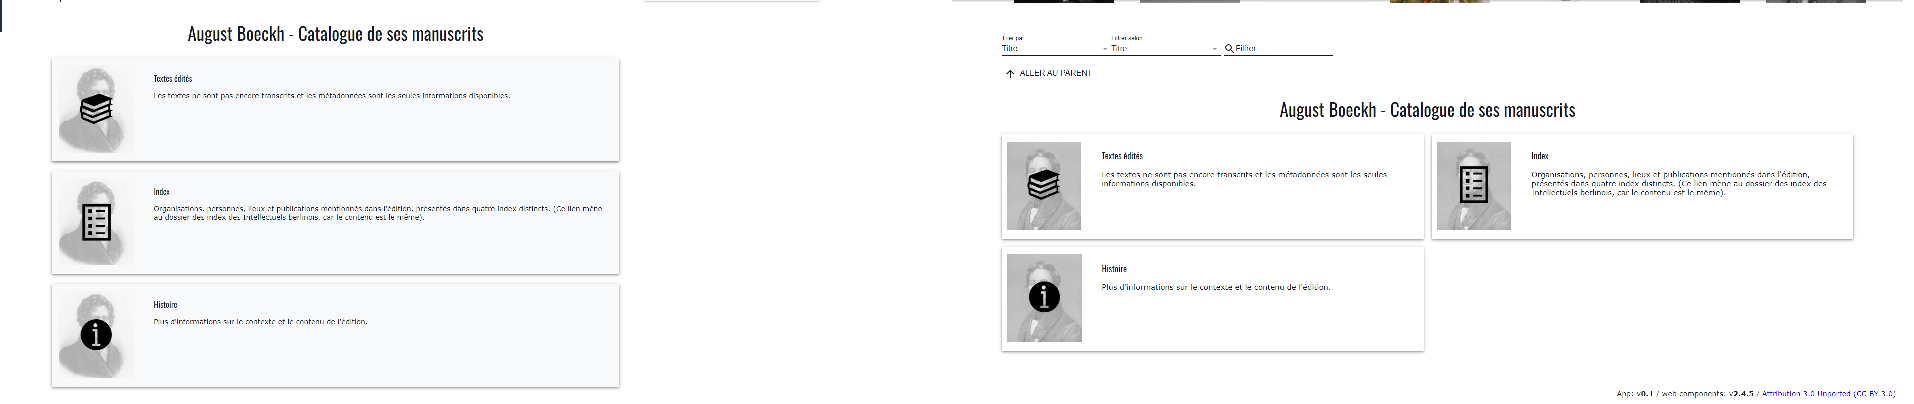
\includegraphics[width=1\linewidth]{schémas/page_corpus.png}
\caption{Les pages de corpus avant (gauche) puis après modifications (droite)}
\label{fig:schémas13}
\end{figure}

Pour mettre en place ces éléments de \textit{design}, seules des compétences de base en HTML sont nécessaires, à l'exception du carrousel, qui requiert des connaissances en JavaScript. TEI Publisher ne propose pas de fonction d'aide pour le HTML, car il nécessite une modification directe des fichiers HTML. Il existe de nombreux projets \textit{open source} qui peuvent servir de source d'inspiration pour des \textit{designs} intéressants, par exemple \href{https://teipublisher.com/exist/apps/vangogh/index.html}{Vincent van Gogh - The Letters
\footcite{VanGoghLetters}}. 

Cependant, il est important de noter que le \textit{design} d'un site web représente un véritable défi, qui devient d'autant plus complexe à mesure que la taille du site augmente. Par conséquent, il peut parfois être nécessaire de faire appel à un web \textit{designer}. L'avantage supplémentaire de travailler avec un web \textit{designer} est la possibilité de rendre le site adaptatif à différentes tailles d'écran, y compris les smartphones.

Un autre point pas encore abordé est le \textit{design} des éléments TEI Publisher qui proviennent du \textit{bundle}. Grâce à la documentation, nous avons à notre disposition des variables CSS pour modifier le \textit{design} des <pb-elements> (comme \textit{--pb-timeline-height}, qui permet de modifier la hauteur de la \textit{timeline}). Les variables mises à notre disposition ont été choisies par TEI Publisher et sont immuables. C'est l'une des raisons pour laquelle les sites TEI Publisher se ressemblent : le \textit{bundle} n'autorise pas une liberté assez grande pour pouvoir produire un \textit{design} propre à notre application. Le \textit{bundle} est contrôlé par TEI Publisher. Pour l'utiliser, il faut charger le fichier JavaScript depuis Internet, il est donc externe à notre application. Il existe une documentation dans la \href{https://faq.teipublisher.com/}{FAQ\footcite{FrequentlyAskedQuestions}} qui propose, à partir du \textit{bundle}, de modifier le \textit{bundle} en local et de développer ses propres éléments ou de modifier les existants. Le <pb-timeline> de DiScholEd devrait utiliser un \href{https://gitlab.inria.fr/dh-projects/discholed/-/blob/main/Pb-component-bundle/pb-timeline.js}{\textit{bundle} personnalisé\footcite{FilesMainDHprojects2023}}, mais nous n'avons pas réussi à le mettre en place pendant le stage. Le \textit{design} peut donc être modifié en profondeur mais demande de fortes connaissances en développement ou alors de faire appel à une société de \textit{design} comme les éditions numériques de la \textit{Bibliotheca Hertziana}: \og{}\textit{a complete re-\textit{design} with the support of a \textit{design} company}\fg{}\footcite{epapers4200}..\\

Nous avons choisi TEI Publisher parce que c'est un CMS dédié aux éditions numériques et qu'il est accessible aux non-développeurs. Cependant, à travers les différents problèmes de \textit{bugs}, la mise en place de nouvelles fonctionnalités et l'amélioration générale de l'application, il semble que de nombreux problèmes apparaissent, soulevant de nouveaux défis et questionnements. Comme nous l'avons également observé, plus notre application est grande, plus les problèmes sont fréquents et difficiles à résoudre. Chaque nouveau corpus ajoute des documents avec des encodages qui ne sont parfois pas adaptés à notre ODD et demande une refonte d'une partie de l'ODD spécialement pour ce corpus. Le \textit{low-code} nous permet d'utiliser des balises personnalisées du \textit{bundle} et de l'interface graphique de l'ODD. Cependant il est nécessaire, vu la taille de notre application, d'aller directement dans les fichiers pour modifier manuellement le \textit{design} et l'ODD. Nous pouvons alors émettre l'hypothèse que le \textit{low-code} devient donc obsolète à mesure que l'application grandit, cependant son obsolescence est due à deux facteurs : une variation de l'encodage des fichiers et un \textit{bundle} qui restreint fortement le \textit{design} général. 